%----------------------------------------------------------------------------------------
%	SECTION 1
%----------------------------------------------------------------------------------------

\section{Science and Mathematics (SM)}

\subsection*{SM1(i, b, m)}

\begin{wraptable}{r}{0.2\textwidth}
	\begin{tabular}{|ll|}
		\hline
		\multicolumn{2}{|c|}{\cellcolor[HTML]{F8A102}\textbf{SM1(i, b, m) \nomaster}} \\ \hline
		\ConTechOne & \BST \\
		\MechB & \ConTechTwo \\
		\Acoustics & \HYD \\
		\Stats & \EPA \\
		\ELS & \TPS \\
		\LAB & \WSD \\
		Arup &  \\ \hline
	\end{tabular}
\end{wraptable}

Multiple courses (mainly from years 2 and 3) have contributed to my knowledge and understanding of scientific principles and methodology necessary to underpin my education in Architectural Engineering.
A main contributor was \textit{Thermal Performance Studies}.
On this course I learned the scientific principles of psychrometrics, i.e. the properties of air-vapour mixtures (like air), and how to use this knowledge in the design of air conditioners, heat exchangers and cooling towers.
Learning about the environmental effects of refrigerants has contributed to my understanding of the evolution of air conditioners, from using carbon- and fluoride-based refrigerants to water and eventually PCMs like Sunamp uses.

Learning the scientific principles of related disciplines h as helped me enrich my appreciation of the scientific and engineering context of my discipline.
\textit{Statistics for Science} has, for example, helped me understand the proper methodology behind sampling populations and to identify bias in data.
\textit{Hydraulics and Hydrology A}, a civil engineering course, helped me appreciate the hydrological cycle (relevant to rainwater and urban drainage) and water flow in pipes (relevant to drainage, water supply and heating systems).








\subsection*{SM2(i, b, m)}

\begin{wraptable}{r}{0.2\textwidth}
	\begin{tabular}{|ll|}
		\hline
		\multicolumn{2}{|c|}{\cellcolor[HTML]{F8A102}\textbf{SM2(i, b, m) \nomaster}} \\ \hline
		\MESOne & \MESTwo \\
		\EnvBeh & \Stats \\
		\TPS & \LAB \\ \hline
	\end{tabular}
\end{wraptable}

\textit{Mathematics for Engineers and Scientists 1 and 2} and \textit{Statistics for Science} all further developed my knowledge and understanding of mathematical and statistical methods.
I have been able to apply this knowledge in the analysis and solution of engineering problems.
For example, I used it to work out the yield of an array of photovoltaic panels (PV) in \textit{Energy and Buildings} as well as the yield of a set of turbines in a tidal energy generation system as part of my collaborative project in \textit{Design Project} (see more about this under EA6m in Section~\ref{sec:EA6m}).








\subsection*{SM3(b, m)}

\begin{wraptable}{r}{0.2\textwidth}
	\begin{tabular}{|ll|}
		\hline
		\multicolumn{2}{|c|}{\cellcolor[HTML]{F8A102}\textbf{SM3(b, m) \nomaster}} \\ \hline
		\ConTechOne & \MechB \\
		\ConTechTwo & \HYD \\
		\LAB &  \\ \hline
	\end{tabular}
\end{wraptable}

Other engineering disciplines that I have gained knowledge and understanding from are predominantly civil and structural.
%These were acquired through the following courses: \textit{Mechanics B}, \textit{Construction Technology 1 and 2},  and \textit{Hydraulics and Hydrology A}.
%\hl{I cannot remember how I have applied or integrated this knowledge though...
%pipes?
%materials choice?}
I have been able to apply and integrate this knowledge and understanding to support study of my own engineering discipline.
For example, during a computational fluid dynamics (CFD) modelling exercise in the \textit{Laboratory Project}, I was able to identify laminar and turbulent flows, something I had learned about it in \textit{Hydraulics and Hydrology A}.
This enabled me to refine and improve my CFD model.








\subsection*{SM4m}

\begin{wraptable}{r}{0.2\textwidth}
	\begin{tabular}{|ll|}
		\hline
		\multicolumn{2}{|c|}{\cellcolor[HTML]{F8A102}\textbf{SM4m \master}} \\ \hline
		\BST & \DPA \\
		\CAS & \DSA \\
		\EnBldgs & \PRJ \\
		\DST & \ICP \\
		\WSD &  \\ \hline
	\end{tabular}
\end{wraptable}

A range of courses increased my awareness of developing technologies relevant to Architectural Engineering and building services.
In \textit{Building Services Technology}, \textit{Energy and Buildings}, \textit{Dissertation} and \textit{Innovation in Construction Practice}, I respectively learned about technologies such as modern windcatchers, smart meters, BIM and virtual and augmented reality.
I was also exposed to a developing technology during my placement at Sunamp: their PCM-based heat batteries.








\subsection*{SM5m}

\begin{wraptable}{r}{0.2\textwidth}
	\begin{tabular}{|ll|}
		\hline
		\multicolumn{2}{|c|}{\cellcolor[HTML]{F8A102}\textbf{SM5m \littlemaster}} \\ \hline
		\DSA & \LAB \\ \hline
	\end{tabular}
\end{wraptable}

\textit{Design Software Applications} and \textit{Laboratory Project} have made me aware of the mathematical and computational models relevant to Architectural Engineering.
I learned how steady-state and dynamic software applications function and their limitations, and was made aware of the mathematical and computational models they are based on.
I was introduced to and got to practise using the following applications:
\begin{itemize}
    \item Steady-state:
    	\begin{itemize}
    		\item iSBEM (interface for Simplified Building Energy Model)
    		\item SAP (Standard Assessment Procedure)
    		\item PHOENICS, a CFD software application
    	\end{itemize}
    \item Dynamic: IES-VE (Integrated Environmental Solutions - Virtual Environment)
\end{itemize}

I think I would need further practice with the software applications to strengthen my understanding of the associated mathematical and computational models.







\subsection*{SM6m}

\begin{wraptable}{r}{0.2\textwidth}
	\begin{tabular}{|ll|}
		\hline
		\multicolumn{2}{|c|}{\cellcolor[HTML]{F8A102}\textbf{SM6m \nomaster}} \\ \hline
		\HBE & \ID \\
		\BST & \IE \\
		\DPA & \Acoustics \\
		\HYD & \EnvBeh \\
		\CAS & \EnBldgs \\
		\TPS & \DI \\
		\DST & \LAB \\
		\ISE & \ICP \\
		Arup & Hoare Lea \\
		Sunamp &  \\ \hline
	\end{tabular}
\end{wraptable}

I have gained an understanding of concepts from a range of areas, including some outside engineering, and been able to critically evaluate and apply these concepts in my engineering projects.
One instance 
is when I came across a social sciences journal paper about survey research as I conducted a post-occupancy evaluation (POE) for \textit{Environment and Behaviour}.
The paper analysed typical response styles and suggested how to design questionnaires to avoid biased or inaccurate data collection.
Using this information, I was able to critically evaluate the success of the questionnaire used for the POE in \textit{Environment and Behaviour} and design an improved survey questionnaire for the acoustic \textit{Laboratory Project}.

Another instance 
is when I learned about the sustainable design hierarchy (see Figure~\ref{fig_hierarchy}) during my placement at Arup.
I then applied this approach to the design of a library for a group project in \textit{Critical Architectural Studies}, helping us earn the first prize in sustainable design (see Figure~\ref{fig_award}).


\begin{figure}[htbp]
	\centering
	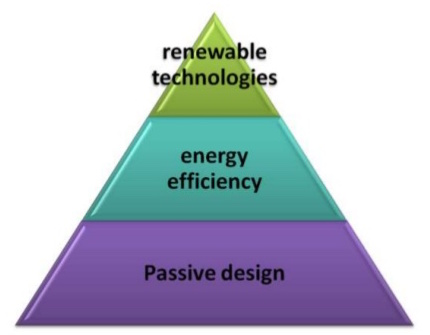
\includegraphics[width=0.3\textwidth]{figures/Hierarchy.jpg}
	\rule{\textwidth}{0.5pt} % use line???
	\caption[The sustainable design hierarchy.]{The sustainable design hierarchy \citep{Dougherty:online}.}
	\label{fig_hierarchy}
\end{figure}


\begin{figure}[htbp]
	\centering
	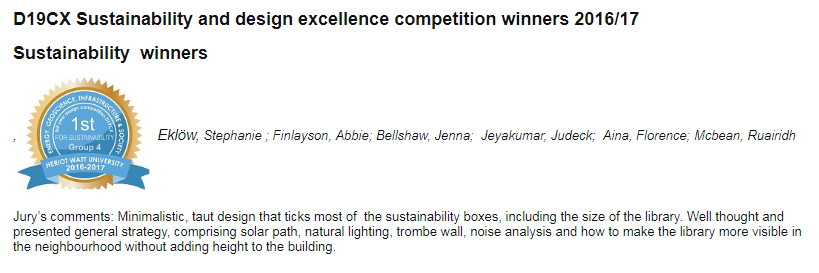
\includegraphics[width=\textwidth]{figures/SustainabilityAward.PNG}
	\rule{\textwidth}{0.5pt} % use line???
	\caption[First prize for sustainability awarded to my group for our library design in D19CX.]{First prize for sustainability awarded to my group for our library design in \textit{Critical Architectural Studies} (D19CX).}
	\label{fig_award}
\end{figure}

